%
%  untitled
%
%  Created by Johan Boissard [] on 2010-06-24.
%  Copyright (c) Johan Boissard. All rights reserved.
% hhh

\documentclass[a4paper] {scrartcl}
\usepackage[T1]{fontenc}
\usepackage[utf8]{inputenc}
\usepackage{graphicx}
\usepackage{engord}
%\usepackage[english]{babel}
\usepackage{fancyhdr}
\usepackage{amsmath}
\usepackage{comment}

\usepackage{listings}

%allows inclusion of url (hyperref is better than url) 
%ref: http://www.fauskes.net/nb/latextips/
\usepackage{hyperref}

%package for chemistry ie: \ce{(NH4)2SO4 -> NH4+ + 2SO4^2-} 
%ref:www.ctan.org/tex-archive/macros/latex/contrib/mhchem/mhchem.pdf
\usepackage[version=3]{mhchem}
%celsius + degrees
\usepackage{gensymb}
%to get last page
\usepackage{lastpage} % \pageref{LastPage}

%make use of the fullpage (no HUGE margins)
\usepackage{fullpage}
\usepackage{subfig}

%allows separating cell in table by diagonal line
\usepackage{slashbox}




%\renewcommand{\chaptername}{Laboratory}
%\setcounter{chapter}{5}

\usepackage{color}
\usepackage[usenames,dvipsnames, table]{xcolor}
% Include this somewhere in your document



\usepackage[absolute]{textpos}

%column  of multi row in tables
\usepackage{multirow}

%to have vertical text in table
\usepackage{rotating}


%%%%%%% a virer ici!!!!
\begin{comment}
%Fonts and Tweaks for XeLaTeX
\usepackage{fontspec,xltxtra,xunicode}
%\defaultfontfeatures{Mapping=tex-text}
%\setromanfont[Mapping=tex-text]{Hoefler Text}
\setsansfont[Scale=MatchLowercase,Mapping=tex-text]{Gill Sans}

\definecolor{shade}{HTML}{D4D7FE}	%light blue shade
\definecolor{text1}{HTML}{272727}		%text is almost black
\definecolor{headings}{HTML}{173849} 	%dark blue %%%dark red 70111
\definecolor{title}{HTML}{173849} 	%dark blue %%%dark red 70111

\usepackage{titlesec}				%custom \section
\end{comment}







\author{Johan Boissard}
\date{\today}
\title{Accounting}
\begin {document}

\maketitle
%\tableofcontents
%\twocolumn
%\chapter{Microeconomics}

%1 week
\section{Introduction}
\begin{enumerate}
	\item Opening of the accounts: balance sheet to accounts (01.01)
	\item Recording of transactions
	\begin{itemize}
		\item Assets and liabilities + equity
		\item expenses and revenues
	\end{itemize}
	\item Closing: accounts to \textbf{balance sheet} and \textbf{income statement} (31.12)
\end{enumerate}

\subsection{Terminology}
\begin{itemize}
	\item Debit: that which is owed
	\item Debtor: owes money to somebody (receivables)
	\item Credit: that which is loaned
	\item Creditor: somebody whom money is owed (payables)
\end{itemize}

In the banking system, it is the \underline{opposite}!

\section{Accounts}
\begin{sidewaystable}
\centering
\begin{tabular}{l|c|c || c | c}
	&\multicolumn{2}{c||}{\textbf{Position accounts}}&
	\multicolumn{2}{c}{\textbf{Performance accounts}}\\
	
	&\multicolumn{2}{c||}{Never set to $0$}&
	\multicolumn{2}{c}{Set to $0$ every beginning of year}\\
	
	\hline
	&\textbf{assets} & \textbf{liabilities} & \textbf{expense }& \textbf{revenues}\\
	&actifs & passifs & charges & produits\\
	\hline
	Def &items belonging to the company & debts of company (+capital) 
	& expenses during year & revenues during year
	\\
	&debit-credit & credit-debit & debit-credit & credit-debit\\
	&+/- & -/+ & +/- & -/+\\
	Increase & debit side & credit side& debit side &credit side\\
	Decrease&credit side &debit side& credit side & debit side\\
	OB & from balance sheet & from balance sheet & $0$ & $0$\\
	EB & to balance sheet & to balance sheet & to income statement & to income statement\\
	\hline
	Examples&Cash & Payables & Cost of sale & Sales revenues\\
	&Receivables   & Bank Loan & Salary & Interest revenues\\
	&Inventories & \textbf{Equity} & Rent & \\
	&Equipment  &		& Energy  &\\
	&Land && Maintenance&\\
	& VAT input taxes & VAT output taxes &&
\end{tabular}
\caption{Summary of the different accounts and their properties}
\end{sidewaystable}

\subsection{Double-entry accounting}
\textbf{For every debit entry, there must be a corresponding credit entry of the same amount}

\paragraph{Example of transaction:}
Equipment to Cash 1000, (means "Purchase of a machine for $1'000$ CHF)\\\\
\begin{tabular}{lllrl}
	\textbf{debit} & & \textbf{credit} & \textbf{amount} [CHF]&\\
	\hline
	Equipment & / & Bank & 1000&
\end{tabular}


\subsection{Journal and Ledger}
The \textbf{Journal} is a chronological record of business transactions during a given period.

The \textbf{Ledger} contains the individual accounts.


\section{Balance sheet and Income sheet}
\subsection{Balance sheet (Bilan)}
The balance sheet is made up of 2 sides: assets \& liabilities + equity
\subsubsection{Assets}
The assets column is organized as follows:


\begin{enumerate}
	\item current assets
	\begin{enumerate}
		\item cash and cash equivalents (post, bank accounts)
		\item marketable securities
		\item accounts receivable (debtors)
		\item inventory (stock)
		\item prepayments
	\end{enumerate}
	\item fixed assets
	\begin{enumerate}
		\item Equipment, vehicles, furniture, fixtures and fittings
		\item Investment
		\item Land and Building
	\end{enumerate}
\end{enumerate}
This should represent the \textbf{order of liquidity}.

\subsubsection{Liabilities + equity}
This column is organized as follows:
\begin{enumerate}
	\item short-term (or current) Liabilities (less than one year turn-over)
	\begin{enumerate}
		\item Bank current account
		\item Accounts payable (creditors)
		\item Short-term provision
		\item Accruals
	\end{enumerate}
	\item long-term (or non-current) liabilities (more than one-year turn-over)
	\begin{enumerate}
		\item Mortgage
		\item Debenture
		\item Long-term provision
	\end{enumerate}
	\item equity (capital + shares of company)
	\begin{enumerate}
		\item Share capital
		\item Reserves
		\item Retained earnings
	\end{enumerate}
\end{enumerate}



\subsection{The "accounting equation"}
\begin{eqnarray}
	\text{Total assets} = \text{Total liabilities} +\text{Equity}
\end{eqnarray}
Amount in left column equals amount on right column.

\subsection{Income statement (Compte de résultats)}
\begin{enumerate}
	\item Provides informations on the profit or loss of the company
	\item has a balance of $0$ at the beginning of the year
	\item is a summary of the expenses and revenues accounts at closing
	\item The \textbf{result} is transferred to the balance sheet
\end{enumerate}

\begin{eqnarray}
	\text{Gross-profit} &=& \text{Sales revenues}- \text{Cost of goods sold}\\
	\text{Operating profit} &=& \text{Gross profit}- \text{Operating costs}\\
	\text{Net income} &=& \text{Operating profit} \pm \text{Non-operating performance}
\end{eqnarray}

\subsection{The accounting cycle}
starts with a balance sheet at the beginning of the period and ends with a balance sheet at the end of the period.


%%% week 3 %%%
\section{Merchandising and inventories}
Two different ways to record it:

\begin{tabular}{lllllrl}
	&\multicolumn{3}{l}{\textbf{Perpetual inventory system}} 
	& \multicolumn{3}{l}{\textbf{Periodic inventory system}}\\
	\hline
	&\multicolumn{6}{c}{Purchase of 10 items at 2'000 CHF each} \\
	%purchase&"inventory" (assets) used &"cost of sales" (expense) used\\
	purchase 
		& inventory/& cash& 20'000 
		&cost of sale/& cash& 20'000	\\
		&\multicolumn{6}{c}{Sale of 6 items at 3'000 CHF each} \\
	sales 
		& cash/& sales revenue & 18'000
		& cash/& sales revenue& 18'000\\
	& cost of sale /& inventory & 12'000\\
	&\multicolumn{6}{c}{Physical inventory 4 items at 2000 CHF each}\\
	adjustment &&& & inventory/& cost of sales& 8'000\\
	\hline
%	& \multicolumn{3}{l}{no adjustments} & \multicolumn{3}{l}{needs to be adjusted}
\end{tabular}

\subsection{Variations of cost of sales}
\subsubsection{FIFO (first in first out)}
First that came in ($\text{price}_0$) is the first to go.

\subsubsection{LIFO (last in first out)}
Last that came in ($\text{price}_0$) is the first to go. (preferred method in Switerland)
\subsubsection{Weighted average cost}
Average cost of the good bought.

\section{Drawing account}



\section{VAT - Value Added Tax (TVA)}
\subsection{VAT}
VAT is a general consumption tax on goods and services. It covers all goods and services that are not expressly exempted from tax.
\subsubsection{Goods and services exempted from tax}
\begin{enumerate}
	\item Postal-services
	\item All health care services
	\item Educational and training services
	\item most sporting and cultural services (theatre, music)
	\item Insurance transactions
	\item Most bank transactions
	\item Changes in ownership of buildings and land (housing)
\end{enumerate}

\subsubsection{VAT rates}
\begin{tabular}{|l|l|l|}
	\hline
	Standard rate & 8.0\% & \\
	\hline
	Reduced rate & 2.5\% & food, beverage, books, newspapers..\\
	\hline
	Special rate & 3.8\%& accommodations (hotels)\\
	\hline
\end{tabular}


\subsubsection{Purchase of a good}

\paragraph{Example of transaction:}
\begin{tabular}{lllrl}
	\textbf{debit} & & \textbf{credit} & \textbf{amount} [CHF]&\\
	\hline
 	Cost of sales & / & &300&\\
	Vat input&/ & & 24&\\
	&/ &Payables & 324&
\end{tabular}


\subsubsection{Sale of a good}

\paragraph{Example of transaction:}
\begin{tabular}{lllrl}
	\textbf{debit} & & \textbf{credit} & \textbf{amount} [CHF]&\\
	\hline
	Receivables & / & &1080&\\
	&/ &Sales revenues & 1000&\\
	&/ &VAT out & 80&
\end{tabular}

\subsubsection{Settlement}

\paragraph{Example of transaction:}
\begin{tabular}{lllrl}
	\textbf{debit} & & \textbf{credit} & \textbf{amount} [CHF]&\\
	\hline
	VAT out & / & VAT in &8&\\
	VAT out &/ & Cash & 16&
\end{tabular}

\section{Discounts}
\paragraph{Example of transaction:}


Payment of suppliers' invoice $81'000$ CHF under deduction of $2\%$\\

\begin{tabular}{lllrl}
	\textbf{debit} & & \textbf{credit} & \textbf{amount} [CHF]&\\
	\hline
	Payables & / &  & $81'000$&\\
	 & / & Bank  & $79'380$&$=81'000\cdot0.98$\\
	 & / & Cost of Sales  & $1'500$&$=(81'000-79'380)\cdot\frac{100}{108}$\\
	 & / & VAT \underline{input} tax  & $120$&$=(81'000-79'380)\cdot\frac{8}{108}$\\
\end{tabular}


\paragraph{Example of transaction:}


debtor settle invoice $54'000$ CHF less $2\%$ by paying into bank account\\

\begin{tabular}{lllrl}
	\textbf{debit} & & \textbf{credit} & \textbf{amount} [CHF]&\\
	\hline
	 & / & Receivables & $54'000$&\\
	 Bank & / &  & $52'920$&$=54'000\cdot0.98$\\
	 Sales revenue & / & & $1'000$&$=(54'000-52'920)\cdot\frac{100}{108}$\\
	 VAT \underline{output} tax & / &  & $80$&$=(54'000-52'920)\cdot\frac{8}{108}$\\
\end{tabular}

\section{Securities}
\paragraph{Example of transaction:}


Purchase of securities $20'000$ CHF, bank fees $300$ CHF.\\

\begin{tabular}{lllrl}
	\textbf{debit} & & \textbf{credit} & \textbf{amount} [CHF]&\\
	\hline
	 & / & Bank & $20'300$&\\
	 Securities & / &  & $20'000$&\\
	 Securities expenses & / &   & $300$&\\
\end{tabular}


\paragraph{Example of transaction:}


sale of the securities $24'000$ CHF, bank fees $320$ CHF\\

\begin{tabular}{lllrl}
	\textbf{debit} & & \textbf{credit} & \textbf{amount} [CHF]&\\
	\hline
	Securities & / & Securities revenues & $4'000$&\\
	 Bank & / &  & $23'680$&\\
	 Securities expense & / &  & $320$&\\
	  & / & Securities & $24'000$&\\
\end{tabular}

\underline{Note:} ne pas oublier la ligne de revenu de la sécurité, sinon la balance ne joue plus.

\section{Accruals}
4 accounts
\begin{itemize}
	\item Accrued revenues (receivable/débit), ce que l'entreprise va recevoir, mais pour lequel elle n'a pas encore émis de facture ou intérêt à recevoir. Prendre en compte l'année en cours
	\item Accrued expenses and deferred values (payable/crédit), ce que l'entreprise doit payer, mais dont la facture n'a pas encore été émise ou intérêt à payer. Prendre en compte l'année en cours
	\item Prepaid expenses (receivable/débit). Ce qui a déjà été payé. Prendre en compte l'année suivante.
	\item Deferred revenues (payable/crédit). 
\end{itemize}

\underline{They appear at beginning and end of year.}

\paragraph{example} Securities ($90'000$) made of bonds of the firm ABB, $4\%$ due on 31.10.\\

\begin{tabular}{lllrl}
	\textbf{debit} & & \textbf{credit} & \textbf{amount} [CHF]&\\
	\hline
	Accrued revenues & / &  Securities revenues & $600$&$ = 90'000\cdot0.04\cdot\frac{2}{12}$\\
\end{tabular}

\paragraph{example} Bank loan $400'000$ CHF, interest $5\%$ payable 31.03 and on 30.09\\

\begin{tabular}{lllrl}
	\textbf{debit} & & \textbf{credit} & \textbf{amount} [CHF]&\\
	\hline
	 Securities expenses & / &  Accrued expenses & $5'000$&$ = 400'000\cdot0.05\cdot\frac{3}{12}$\\
\end{tabular}

\section{Withholding tax}
La taxe avant impôt (peut être récupérée si déduite).

\paragraph{example} Collection of the interest coupons on bonds of the firm ABB ($90'000$ at $4\%$). The withholding tax amount is $35\%$\\

\begin{tabular}{lllrl}
	\textbf{debit} & & \textbf{credit} & \textbf{amount} [CHF]&\\
	\hline
	Bank & / &   & $2'340$&$ =3'600-1'260$\\
	Debtor Withholding Tax & / &  & $1'260$&$ =3'600\cdot0.35$\\
	 & / &  Securities revenues & $3'600$&$ = 90'000\cdot0.04$\\
\end{tabular}

\section{Provisions}
\begin{itemize}
	\item taxes: tax expenses / provisions for taxes
	\item guarantees: guarantees expenses / provisions for guarantees
	\item bad debts: loss on receivable / provision on bad debts
\end{itemize}

La dissolution de provision se fait dans le compte inverse si on est dans la même année sinon dans \textbf{extraordinary revenues}. Page 6 cours 5.

\paragraph{example} A provision for guarantee of $10'000$ CHF \\

\begin{tabular}{lllrl}
	\textbf{debit} & & \textbf{credit} & \textbf{amount} [CHF]&\\
	\hline
	 Guarantee expenses & / &  Provisions for guarantee & $10'000$\\
\end{tabular}

\paragraph{example} The provision for currency risks of $200'000$ can be reduced by $50'000$ CHF at year-end.\\

\begin{tabular}{lllrl}
	\textbf{debit} & & \textbf{credit} & \textbf{amount} [CHF]&\\
	\hline
	 Provisions for currency risks & / &  Extraordinary revenues & $50'000$\\
\end{tabular}

\section{Depreciation}
2 types of depreciation
\begin{itemize}
	\item direct $\rightarrow$ depreciation expenses / machine
	\item indirect $\rightarrow$ depreciation expenses / accumulated depreciation
\end{itemize}

\subsection{Methods for calculating depreciation}
\subsubsection{Straight line method}
	\begin{enumerate}
		\item set duration of machine
		\item every year reduce by $\frac{\text{price of mschine}}{\text{duration}}$
	\end{enumerate}
	\paragraph{Example} % (fold)
	\label{par:example}
	purchase of a machine for $10'000$ CHF, residual value after $5$ years: $0$ CHF.
	$\Rightarrow$ Every year $\frac{10000}{5}=2000$ CHF less value.
	% paragraph example (end)
	
	
\subsubsection{Reducing balance method}
\begin{enumerate}
	\item set rate: double the rate of the striaght line method (in our example $2\cdot\frac{2000}{10000}=.4=40\%$)
	\item reduce the price by $40\%$.
\end{enumerate}
\paragraph{Example} % (fold)
\label{par:example}
purchase of a machine for $10'000$ CHF, residual value after $5$ years: $0$ CHF.

\begin{tabular}{|c|c|c|}
	\hline
	year & book value & depreciation\\
	0 & $100'000$ & \\
	1 & $60'000$ & $40'000$\\
	2 & $36'000$ & $24'000$\\
	3 & $21'600$ & $14'400$\\
	4 & $12'960$ & $8'640$\\
	5 & $7'776$ & $5'184$\\
	\hline
\end{tabular}
% paragraph example (end)

\subsection{example} 
\begin{enumerate}
	\item on 01.01.2001 cash acquisition of 2 machines for $100'000$ CHF each
	\item on 31.12.2001 depreciation $40\%$ of the book value 
	\item on 31.03.2002 sale ofone machine for $70'000$ CHF cash
	\item on 31.12.2002 depreciation $40\%$ from the book value
	\item on 01.07.2003 sale of the $2^{\text{nd}}$ machine for $25'000$ CHF cash
\end{enumerate}

Direct method:

\begin{tabular}{lllllrl}
	&\textbf{debit} & & \textbf{credit} & \textbf{amount} [CHF]&\\
	\hline
	1&Machinery & / &  Cash & $200'000$&$=2\cdot100'000$\\
	2&Depreciation expenses& / & Machinery & $8'000$&$=2\cdot100'000\cdot0.4$\\
	3&Depreciation expenses& / & Machinery & $6'000$&$=(100'000\cdot(1-0.4))\cdot0.4\cdot\frac{3}{12}$\\
	&Cash& / & Machinery & $54'000$&$=60'000-6'000$\\
	&Cash& / & Extra. revenues & $16'000$&$=70'000-54'000$\\
	
	4&Depreciation revenues& / & Machinery & $24'000$&$=60'000\cdot0.4$\\
	5&Depreciation revenues& / & Machinery & $7'200$&$=(60'000-24'000)\cdot0.4\cdot\frac{6}{12}$\\
	&Cash& / & Machinery & $28'800$& $=36'000-7'200$\\
	&Book loss& / & Machinery & $3'800$& $=28'800-25'000$\\
\end{tabular}

Indirect method:

\begin{tabular}{lllllrl}
	&\textbf{debit} & & \textbf{credit} & \textbf{amount} [CHF]&\\
	\hline
	1&Machinery & / &  Cash & $200'000$&$=2\cdot100'000$\\
	2&Depreciation expenses& / & Acc. dep. & $8'000$&$=2\cdot100'000\cdot0.4$\\
	3&Depreciation expenses& / & Acc. dep. & $6'000$&$=(100'000\cdot(1-0.4))\cdot0.4\cdot\frac{3}{12}$\\
	&Acc. dep& / & Dep. dep. & $46'000$&$=40'000+6'000$\\
	&Cash& / & Machinery & $54'000$&$=60'000-6'000$\\
	&Cash& / & Extra. revenues & $16'000$&$=70'000-54'000$\\
	
	4&Depreciation revenues& / & Acc. dep. & $24'000$&$=60'000\cdot0.4$\\
	5&Depreciation revenues& / & Acc. dep. & $7'200$&$=(60'000-24'000)\cdot0.4\cdot\frac{6}{12}$\\
	&Acc. dep& / & Dep. dep. & $71'200$&$=40'000+24'000+7'200$\\
	&Cash& / & Machinery & $28'800$& $=36'000-7'200$\\
	&Book loss& / & Machinery & $3'800$& $=28'800-25'000$\\
\end{tabular}

\section{Evaluation}
\subsection{Principle of prudence} % (fold)
\label{sub:principle_of_prudence}
\begin{itemize}
	\item Book \textbf{gains} are recorded \textbf{after} they have been realised
	\item Book \textbf{losses} are recorded \textbf{before} they are definitely realised
\end{itemize}

For instance, some shares by the company do a good performance: book value do not change
If they do bad, they are recorded at the average value of the month preceding the closing.

\paragraph{Valuation of work in progress and finished goods inventory} % (fold)
\label{par:valuation_of_work_in_progress_and_finished_goods_inventory}

Tableau exemple for homogenous production
\\

\begin{tabular}{| l|c|c|c|c|c|}
	\hline
	 & Items & \% of completion & Total items & Cost per item & Overall costs\\
	\hline
	Beg. balance & $3'500$ & $80\%$ & $2'800$ & $150$ CHF & $420'000$ CHF\\
	\hline
	Ending balance & $6'000$ & $30\%$ & $1'800$ &$150$ CHF & $270'000$ CHF\\
	\hline\hline
	Reduction in inventory & & & & & $150'000$ CHF\\
	\hline
\end{tabular}



Tableau exemple for heterogenous production
\\
\begin{figure}[htbp]
	\centering
		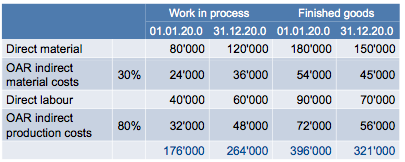
\includegraphics[height=1.7in]{images/heteroProd.png}
	\caption{heterogenous production}
	\label{fig:images_heteroProd}
\end{figure}

\paragraph{exemple} of entry for the previous table % (fold)
\label{par:exemple}

% paragraph exemple (end)
\begin{tabular}{lllrl}
	\textbf{debit} & & \textbf{credit} & \textbf{amount} [CHF]&\\
	\hline
	 Work in Process inventory & / &  Inventory Adjustments & $88'000$&$=264'000-176'000$\\
	 Inventory adjustments & / &  Finished goods inventory & $75'000$&$=396'000-321'000$\\
\end{tabular}



% paragraph valuation_of_work_in_progress_and_finished_goods_inventory (end)

% subsection principle_of_prudence (end)
% paragraph  (end)

\end{document}
